\chapter{Doppler Ultrasound}
\label{ch:ch15_doppler}

% Chapter-opening illustrated modality infographic.
\begin{center}
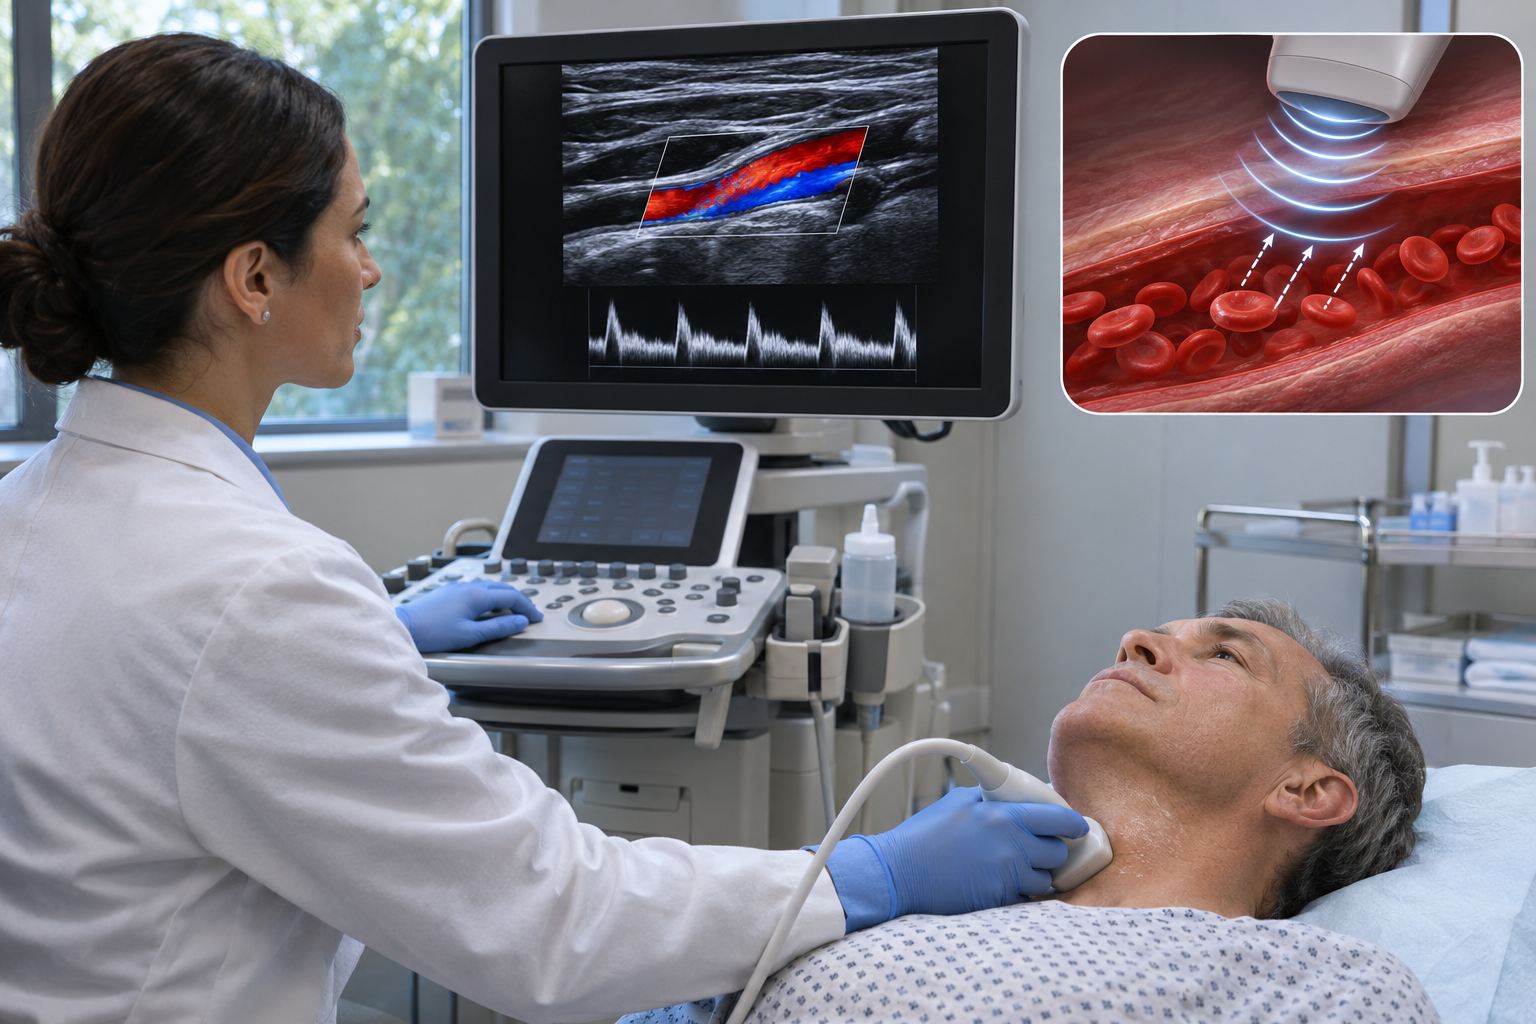
\includegraphics[width=\textwidth,keepaspectratio]{modalities/infographics/doppler_realistic.png}
\end{center}
\begin{center}\footnotesize Doppler measures frequency shifts from moving blood cells to estimate flow direction and velocity; angle and instrument settings affect the result. AI-generated illustration; displayed waveforms and images are illustrative.\end{center}

\section{Overview}
Doppler ultrasound is a specialized ultrasound imaging technique that evaluates the direction, velocity, and characteristics of blood flow through arteries, veins, and cardiac structures. It is particularly useful for identifying vascular obstruction, thrombosis, stenosis, abnormal vascular connections, and impaired tissue perfusion.

This catalogue focuses on diseases and conditions for which Doppler ultrasound provides clinically significant diagnostic information. It includes color Doppler, spectral Doppler, power Doppler, and duplex ultrasonography.

The 142 entries form a preliminary catalogue of diseases, conditions, and hemodynamic abnormalities. Doppler findings depend on acquisition angle, settings, physiologic state, and quantitative criteria. Absent flow does not always prove occlusion, and increased velocity or vascularity does not by itself establish stenosis or malignancy. Some findings require confirmatory imaging, laboratory testing, or clinical assessment.

\section{Where Doppler ultrasound is used}
The following numbered entries present common diagnostic applications by anatomical system. Findings are examples. Doppler measurements should be obtained with appropriate technique and interpreted with anatomy, clinical presentation, and relevant quantitative criteria. A technically limited or negative examination may not exclude disease.

\subsection{Carotid and cerebral circulation}
\begin{enumerate}[leftmargin=*,itemsep=0.45em,topsep=0.4em]
\item \textbf{Carotid artery dissection.} Useful imaging findings include: Possible intimal flap, mural hematoma, or abnormal flow; CTA or MRA may be needed.
\item \textbf{Carotid artery occlusion.} Useful imaging findings include: No detectable flow on a technically adequate examination; low flow or technical factors can mimic occlusion.
\item \textbf{Carotid artery stenosis.} Useful imaging findings include: Velocity criteria interpreted with plaque, waveform, and Doppler angle.
\item \textbf{Carotid atherosclerosis.} Useful imaging findings include: Plaque formation, disturbed blood flow.
\item \textbf{Cerebral circulatory arrest.} Useful imaging findings include: Characteristic waveforms may support assessment under a validated protocol; Doppler findings alone do not establish brain death.
\item \textbf{Cerebral vasospasm.} Useful imaging findings include: Elevated velocities interpreted with vessel ratios and clinical context; TCD is commonly used for monitoring after subarachnoid hemorrhage.
\item \textbf{Intracranial arterial stenosis.} Useful imaging findings include: Elevated velocities may indicate stenosis but depend on vessel, angle, flow state, and collateral circulation.
\item \textbf{Sickle cell cerebral vasculopathy.} Useful imaging findings include: TCD velocities are used for stroke-risk screening in children with sickle cell disease using validated protocols; thresholds are population- and protocol-specific.
\item \textbf{Subclavian steal syndrome.} Useful imaging findings include: Reversed vertebral arterial flow.
\item \textbf{Vertebral artery occlusion.} Useful imaging findings include: No detectable flow on a technically adequate study; confirm if the result changes management.
\item \textbf{Vertebral artery stenosis.} Useful imaging findings include: Focal velocity elevation with supportive waveform changes; limited visualization may require CTA or MRA.
\end{enumerate}

Intracranial blood flow is examined using transcranial Doppler (TCD).

\subsection{Peripheral arterial system}
\begin{enumerate}[leftmargin=*,itemsep=0.45em,topsep=0.4em]
\item \textbf{Acute limb ischemia.} Useful imaging findings include: Severely reduced or absent distal flow.
\item \textbf{Arterial aneurysm.} Useful imaging findings include: Arterial dilatation with altered flow patterns.
\item \textbf{Arterial bypass graft occlusion.} Useful imaging findings include: Absent graft flow.
\item \textbf{Arterial bypass graft stenosis.} Useful imaging findings include: Increased focal flow velocity.
\item \textbf{Arterial embolism.} Useful imaging findings include: Abrupt interruption of arterial flow.
\item \textbf{Arterial occlusion.} Useful imaging findings include: Absence of detectable blood flow.
\item \textbf{Arterial pseudoaneurysm.} Useful imaging findings include: To-and-fro spectral waveform.
\item \textbf{Arterial stenosis.} Useful imaging findings include: Focal increase in flow velocity.
\item \textbf{Arterial thrombosis.} Useful imaging findings include: Intraluminal thrombus with impaired flow.
\item \textbf{Arteriovenous fistula.} Useful imaging findings include: High-velocity turbulent flow.
\item \textbf{Arteriovenous malformation.} Useful imaging findings include: High-flow vascular channels.
\item \textbf{In-stent restenosis.} Useful imaging findings include: Elevated velocities using stent-specific criteria; native-vessel thresholds may overestimate stenosis.
\item \textbf{Peripheral arterial disease.} Useful imaging findings include: Monophasic waveforms, reduced distal perfusion.
\item \textbf{Popliteal artery entrapment syndrome.} Useful imaging findings include: Provocative maneuvers may reproduce flow reduction, which can also occur in asymptomatic people; correlate with symptoms and anatomic imaging.
\item \textbf{Thoracic outlet syndrome.} Useful imaging findings include: Positional compression may occur in asymptomatic people; interpret with symptoms and examination and distinguish arterial from venous disease.
\item \textbf{Thromboangiitis obliterans.} Useful imaging findings include: Distal segmental occlusions are nonspecific; diagnosis depends on clinical criteria and exclusion of other causes.
\end{enumerate}

\subsection{Peripheral venous system}
\begin{enumerate}[leftmargin=*,itemsep=0.45em,topsep=0.4em]
\item \textbf{Central venous stenosis.} Useful imaging findings include: Abnormal venous flow patterns.
\item \textbf{Chronic venous insufficiency.} Useful imaging findings include: Prolonged retrograde blood flow.
\item \textbf{Deep vein thrombosis (DVT).} Useful imaging findings include: Noncompressibility is the key finding. Doppler flow supports assessment but a negative limited study may require repeat or whole-leg ultrasound.
\item \textbf{Iliac vein thrombosis.} Useful imaging findings include: Abnormal or absent flow may raise suspicion, but pelvic veins can be difficult to visualize; CT or MR venography may be needed.
\item \textbf{Inferior vena cava thrombosis.} Useful imaging findings include: Visible thrombus or absent flow may support diagnosis; ultrasound can be limited by bowel gas and body habitus.
\item \textbf{May--Thurner syndrome.} Useful imaging findings include: Iliac vein compression and altered flow are supportive findings but compression is common without symptoms; assess for clinically significant obstruction and thrombosis.
\item \textbf{Paget--Schroetter syndrome.} Useful imaging findings include: Axillary-subclavian venous thrombosis.
\item \textbf{Post-thrombotic syndrome.} Useful imaging findings include: Residual obstruction and venous reflux.
\item \textbf{Superficial venous thrombosis.} Useful imaging findings include: Intraluminal thrombus.
\item \textbf{Upper extremity venous thrombosis.} Useful imaging findings include: Reduced flow and venous noncompressibility.
\item \textbf{Varicose veins.} Useful imaging findings include: Dilated superficial veins with reflux.
\item \textbf{Venous aneurysm.} Useful imaging findings include: Focal venous dilatation.
\item \textbf{Venous malformation.} Useful imaging findings include: Slow-flow vascular channels.
\end{enumerate}

\subsection{Hepatic and portal circulation}
\begin{enumerate}[leftmargin=*,itemsep=0.45em,topsep=0.4em]
\item \textbf{Budd--Chiari syndrome.} Useful imaging findings include: Hepatic venous outflow obstruction or collateral flow; technically limited examinations may need cross-sectional venography.
\item \textbf{Cavernous transformation of the portal vein.} Useful imaging findings include: Multiple collateral vascular channels.
\item \textbf{Congestive hepatopathy.} Useful imaging findings include: Increased portal venous pulsatility.
\item \textbf{Hepatic arteriovenous malformation.} Useful imaging findings include: Abnormal high-flow vascular connections.
\item \textbf{Hepatic artery stenosis.} Useful imaging findings include: Elevated focal velocity, tardus-parvus waveform.
\item \textbf{Hepatic artery thrombosis.} Useful imaging findings include: Absence of hepatic arterial flow.
\item \textbf{Hepatic vein thrombosis.} Useful imaging findings include: Absent flow or visible thrombus may support outflow obstruction. This overlaps with Budd--Chiari syndrome and is not a separate Doppler pattern.
\item \textbf{Portal hypertension.} Useful imaging findings include: Reversed portal flow or collaterals support portal hypertension; normal direction of flow does not exclude it.
\item \textbf{Portal vein thrombosis.} Useful imaging findings include: Absent or reduced portal flow.
\item \textbf{Splenic vein thrombosis.} Useful imaging findings include: Reduced or absent splenic venous flow.
\item \textbf{TIPS occlusion.} Useful imaging findings include: Absence of detectable shunt flow.
\item \textbf{TIPS stenosis.} Useful imaging findings include: Abnormal shunt velocities.
\end{enumerate}

\subsection{Renal circulation}
\begin{enumerate}[leftmargin=*,itemsep=0.45em,topsep=0.4em]
\item \textbf{Nutcracker syndrome.} Useful imaging findings include: Compression and velocity ratios may support the diagnosis but also occur without symptoms; clinical correlation is essential.
\item \textbf{Renal arteriovenous fistula.} Useful imaging findings include: Turbulent high-velocity flow.
\item \textbf{Renal artery aneurysm.} Useful imaging findings include: Focal vascular dilatation.
\item \textbf{Renal artery occlusion.} Useful imaging findings include: No detectable flow on an adequate examination; low flow and technical limitations can mimic occlusion.
\item \textbf{Renal artery pseudoaneurysm.} Useful imaging findings include: To-and-fro waveform.
\item \textbf{Renal artery stenosis.} Useful imaging findings include: Use validated velocity and renal-to-aortic ratio criteria with waveform assessment; a technically limited study may need CTA or MRA.
\item \textbf{Renal infarction.} Useful imaging findings include: Regional reduction in perfusion is nonspecific; contrast-enhanced CT or MRI is often needed to confirm.
\item \textbf{Renal vein thrombosis.} Useful imaging findings include: Visible thrombus or abnormal venous and arterial waveforms may support the diagnosis; confirm when technically limited.
\item \textbf{Transplant renal artery stenosis.} Useful imaging findings include: Elevated arterial flow velocity.
\item \textbf{Transplant renal vein thrombosis.} Useful imaging findings include: Absent venous flow, reversed arterial diastolic flow.
\end{enumerate}

\subsection{Abdominal and mesenteric circulation}
\begin{enumerate}[leftmargin=*,itemsep=0.45em,topsep=0.4em]
\item \textbf{Abdominal aortic aneurysm.} Useful imaging findings include: Aortic dilatation, possible mural thrombus.
\item \textbf{Abdominal aortic occlusion.} Useful imaging findings include: Absence of detectable aortic flow.
\item \textbf{Aortoiliac occlusive disease.} Useful imaging findings include: Abnormal aortoiliac flow velocities.
\item \textbf{Endoleak following aneurysm repair.} Useful imaging findings include: Doppler may detect sac flow, but a negative examination does not reliably exclude endoleak; CT angiography or other protocol imaging may be required.
\item \textbf{Median arcuate ligament syndrome.} Useful imaging findings include: Respiratory variation in celiac artery compression; anatomic compression is common in asymptomatic people and does not alone establish the syndrome.
\item \textbf{Mesenteric artery occlusion.} Useful imaging findings include: Absent or severely reduced arterial flow.
\item \textbf{Mesenteric artery stenosis.} Useful imaging findings include: Elevated velocities using validated criteria; fasting state, angle, and technical quality affect measurements.
\item \textbf{Mesenteric venous thrombosis.} Useful imaging findings include: Intraluminal thrombus, reduced venous flow.
\end{enumerate}

\subsection{Obstetric and fetal circulation}
\begin{enumerate}[leftmargin=*,itemsep=0.45em,topsep=0.4em]
\item \textbf{Fetal anemia.} Useful imaging findings include: MCA peak systolic velocity interpreted against gestational age; values above 1.5 MoM prompt specialist assessment, not a stand-alone diagnosis.
\item \textbf{Fetal arteriovenous malformation.} Useful imaging findings include: Abnormal high-flow vascular connections.
\item \textbf{Fetal cardiac compromise.} Useful imaging findings include: Abnormal ductus venosus waveforms indicate hemodynamic concern in selected high-risk pregnancies and require specialist interpretation.
\item \textbf{Fetal circulatory redistribution.} Useful imaging findings include: Low MCA resistance or cerebroplacental ratio may indicate redistribution; interpret with gestational age and the full growth assessment.
\item \textbf{Fetal growth restriction.} Useful imaging findings include: Umbilical artery resistance helps assess placental resistance and guide surveillance after growth restriction is identified; it does not establish FGR alone.
\item \textbf{Placenta accreta spectrum.} Useful imaging findings include: Abnormal lacunae and vascular patterns raise suspicion in an at-risk pregnancy; no individual sign excludes or confirms all cases.
\item \textbf{Placental insufficiency.} Useful imaging findings include: Abnormal waveforms support placental dysfunction in context; no single Doppler result establishes the diagnosis.
\item \textbf{Preeclampsia-associated placental dysfunction.} Useful imaging findings include: Increased uterine artery resistance is a risk marker, not a diagnostic test for preeclampsia.
\item \textbf{Twin anemia-polycythemia sequence.} Useful imaging findings include: Discordant MCA peak systolic velocities support diagnosis using validated intertwin criteria.
\item \textbf{Twin reversed arterial perfusion sequence.} Useful imaging findings include: Reversed arterial perfusion.
\item \textbf{Twin-to-twin transfusion syndrome.} Useful imaging findings include: Doppler findings contribute to staging and assessment; diagnosis also uses amniotic fluid and fetal findings in a monochorionic pregnancy.
\item \textbf{Umbilical artery thrombosis.} Useful imaging findings include: Absent flow in one artery may raise suspicion, but technical factors and cord anatomy must be assessed.
\item \textbf{Vasa previa.} Useful imaging findings include: Color and pulsed Doppler can confirm fetal vessels near or over the internal os; distinguish fetal from maternal vessels.
\item \textbf{Vein of Galen malformation.} Useful imaging findings include: High-flow intracranial vascular structure.
\end{enumerate}

\subsection{Female reproductive system}
\begin{enumerate}[leftmargin=*,itemsep=0.45em,topsep=0.4em]
\item \textbf{Corpus luteum cyst.} Useful imaging findings include: Prominent peripheral vascularity.
\item \textbf{Ectopic pregnancy.} Useful imaging findings include: Peripheral vascularity is nonspecific and also occurs around a corpus luteum; identify an extrauterine gestational sac or use serial clinical assessment.
\item \textbf{Endometrial polyp.} Useful imaging findings include: Single dominant feeding vessel.
\item \textbf{Ovarian carcinoma.} Useful imaging findings include: Internal vascularity in a complex mass can increase suspicion but is not specific for malignancy.
\item \textbf{Ovarian torsion.} Useful imaging findings include: Reduced flow supports torsion, but preserved flow does not exclude it because torsion may be partial or intermittent.
\item \textbf{Ovarian vein thrombosis.} Useful imaging findings include: Intraluminal thrombus, absent or reduced flow.
\item \textbf{Pelvic congestion syndrome.} Useful imaging findings include: Dilated pelvic veins with reflux.
\item \textbf{Retained products of conception.} Useful imaging findings include: Endometrial mass and vascularity support the diagnosis but overlap with other causes; correlate with symptoms and pregnancy history.
\item \textbf{Uterine arteriovenous malformation.} Useful imaging findings include: High-velocity, low-resistance flow.
\item \textbf{Uterine artery pseudoaneurysm.} Useful imaging findings include: To-and-fro waveform.
\item \textbf{Uterine fibroids.} Useful imaging findings include: Peripheral vascularity can be seen but varies with fibroid type and degeneration.
\end{enumerate}

Normal ovarian blood flow does not exclude ovarian torsion.

\subsection{Male reproductive system}
\begin{enumerate}[leftmargin=*,itemsep=0.45em,topsep=0.4em]
\item \textbf{Epididymitis.} Useful imaging findings include: Increased epididymal vascularity.
\item \textbf{Epididymo-orchitis.} Useful imaging findings include: Increased testicular and epididymal flow.
\item \textbf{High-flow priapism.} Useful imaging findings include: Increased cavernosal flow supports the diagnosis, often after trauma; interpret with clinical history and spectral measurements.
\item \textbf{Low-flow priapism.} Useful imaging findings include: Reduced cavernosal flow may be present, but urgent clinical assessment takes precedence and Doppler should not delay treatment.
\item \textbf{Orchitis.} Useful imaging findings include: Increased testicular vascularity.
\item \textbf{Testicular abscess.} Useful imaging findings include: Peripheral vascularity with avascular center.
\item \textbf{Testicular carcinoma.} Useful imaging findings include: A solid intratesticular mass is concerning; vascularity is variable and histology establishes tumor type.
\item \textbf{Testicular infarction.} Useful imaging findings include: Regional absence of perfusion.
\item \textbf{Testicular torsion.} Useful imaging findings include: Reduced flow and a twisted cord support torsion; preserved flow can occur in early, partial, or intermittent torsion.
\item \textbf{Varicocele.} Useful imaging findings include: Dilated veins with retrograde flow.
\item \textbf{Vasculogenic erectile dysfunction.} Useful imaging findings include: Penile duplex is performed after pharmacologic stimulation with protocol-specific measurements; resting flow alone is insufficient.
\end{enumerate}

\subsection{Cardiac Doppler echocardiography}
\begin{enumerate}[leftmargin=*,itemsep=0.45em,topsep=0.4em]
\item \textbf{Aortic regurgitation.} Useful imaging findings include: Retrograde diastolic blood flow.
\item \textbf{Aortic stenosis.} Useful imaging findings include: Increased transvalvular flow velocity.
\item \textbf{Atrial septal defect.} Useful imaging findings include: Abnormal interatrial flow.
\item \textbf{Cardiac tamponade.} Useful imaging findings include: Respiratory flow variation and chamber collapse support tamponade physiology, interpreted with clinical status and pericardial findings.
\item \textbf{Constrictive pericarditis.} Useful imaging findings include: Respiratory inflow variation supports constrictive physiology but overlaps with other conditions; combine with tissue Doppler and pericardial findings.
\item \textbf{Left ventricular diastolic dysfunction.} Useful imaging findings include: Tissue Doppler and transmitral flow are interpreted with left atrial and structural measures; no single velocity establishes filling pressure.
\item \textbf{Mitral regurgitation.} Useful imaging findings include: Retrograde systolic blood flow.
\item \textbf{Mitral stenosis.} Useful imaging findings include: Doppler-derived mean gradient depends on heart rate and flow; assess valve area and clinical context.
\item \textbf{Obstructive hypertrophic cardiomyopathy.} Useful imaging findings include: Increased left ventricular outflow velocity.
\item \textbf{Paravalvular leakage.} Useful imaging findings include: Abnormal flow around a prosthetic valve.
\item \textbf{Patent ductus arteriosus.} Useful imaging findings include: Persistent abnormal vascular flow.
\item \textbf{Prosthetic heart valve stenosis.} Useful imaging findings include: Elevated transprosthetic pressure gradient.
\item \textbf{Pulmonary hypertension.} Useful imaging findings include: Echocardiography estimates probability and pressure; right-heart catheterization confirms hemodynamics when required.
\item \textbf{Pulmonary valve regurgitation.} Useful imaging findings include: Retrograde diastolic flow.
\item \textbf{Pulmonary valve stenosis.} Useful imaging findings include: Increased transvalvular velocity.
\item \textbf{Tricuspid regurgitation.} Useful imaging findings include: Retrograde systolic blood flow.
\item \textbf{Tricuspid stenosis.} Useful imaging findings include: Doppler gradient depends on heart rate and flow; integrate valve morphology and other measurements.
\item \textbf{Ventricular septal defect.} Useful imaging findings include: Abnormal interventricular flow.
\end{enumerate}

\subsection{Inflammatory and musculoskeletal conditions}
\begin{enumerate}[leftmargin=*,itemsep=0.45em,topsep=0.4em]
\item \textbf{Active synovitis.} Useful imaging findings include: Increased synovial blood flow.
\item \textbf{Bursitis.} Useful imaging findings include: Increased peripheral vascularity.
\item \textbf{Cellulitis.} Useful imaging findings include: Increased subcutaneous blood flow.
\item \textbf{Enthesitis.} Useful imaging findings include: Increased vascularity at tendon insertions.
\item \textbf{Giant cell arteritis.} Useful imaging findings include: A noncompressible halo on temporal and axillary artery ultrasound supports diagnosis in trained hands; findings depend on timing and expertise and must be interpreted clinically.
\item \textbf{Psoriatic arthritis.} Useful imaging findings include: Synovial and entheseal hypervascularity.
\item \textbf{Rheumatoid arthritis.} Useful imaging findings include: Increased synovial vascularity.
\item \textbf{Soft-tissue abscess.} Useful imaging findings include: Peripheral hypervascularity.
\item \textbf{Tendinopathy.} Useful imaging findings include: Abnormal intratendinous neovascularization.
\item \textbf{Tenosynovitis.} Useful imaging findings include: Increased tendon sheath vascularity.
\end{enumerate}

\subsection{Thyroid and breast conditions}
\begin{enumerate}[leftmargin=*,itemsep=0.45em,topsep=0.4em]
\item \textbf{Breast abscess.} Useful imaging findings include: Peripheral hypervascularity.
\item \textbf{Breast carcinoma.} Useful imaging findings include: Doppler vascularity is nonspecific; grayscale morphology and clinical findings guide assessment, and biopsy establishes histology.
\item \textbf{Graves disease.} Useful imaging findings include: Diffuse hypervascularity can support Graves disease but is not specific; thyroid function and antibody tests establish the clinical diagnosis.
\item \textbf{Hashimoto thyroiditis.} Useful imaging findings include: Variable thyroid vascularity.
\item \textbf{Intraductal papilloma.} Useful imaging findings include: A vascular stalk supports an intraductal mass but is not specific; pathology may be needed depending on imaging and clinical findings.
\item \textbf{Mastitis.} Useful imaging findings include: Hyperemia can support inflammation but overlaps with other causes; assess for abscess and correlate with symptoms.
\item \textbf{Parathyroid adenoma.} Useful imaging findings include: Prominent polar feeding vessel.
\item \textbf{Thyroid nodules.} Useful imaging findings include: Doppler vascularity alone does not reliably distinguish benign from malignant nodules; use validated grayscale risk stratification and biopsy criteria.
\end{enumerate}

\subsection{Summary}
\begin{center}
\begin{tabular}{@{}p{0.70\textwidth}r@{}}
\toprule
\textbf{Disease category} & \textbf{Entries} \\
\midrule
Anatomical system & Conditions \\
Abdominal and mesenteric circulation & 8 \\
Cardiac Doppler echocardiography & 18 \\
Carotid and cerebral circulation & 11 \\
Female reproductive system & 11 \\
Hepatic and portal circulation & 12 \\
Inflammatory and musculoskeletal conditions & 10 \\
Male reproductive system & 11 \\
Obstetric and fetal circulation & 14 \\
Peripheral arterial system & 16 \\
Peripheral venous system & 13 \\
Renal circulation & 10 \\
Thyroid and breast conditions & 8 \\
Total & 142 \\
\bottomrule
\end{tabular}
\end{center}

\subsection{Types of Doppler imaging}
\begin{longtable}{@{}p{0.34\textwidth}p{0.60\textwidth}@{}}
\toprule
\textbf{Technique} & \textbf{Primary diagnostic application} \\
\midrule
\endfirsthead
\toprule
\textbf{Technique} & \textbf{Primary diagnostic application} \\
\midrule
\endhead
Color Doppler & Blood flow distribution and direction \\
Continuous-wave Doppler & Measurement of high-velocity blood flow \\
Duplex ultrasound & Combined grayscale imaging and Doppler assessment \\
Power Doppler & Detection of slow blood flow \\
Pulsed-wave Doppler & Flow velocity measurement at a specific location \\
Tissue Doppler & Measurement of myocardial tissue velocity \\
Transcranial Doppler & Intracranial blood flow assessment \\
Triplex ultrasound & Grayscale, color, and spectral Doppler \\
\bottomrule
\end{longtable}

\subsection{Authoritative medical sources}
\begin{longtable}{@{}p{0.40\textwidth}p{0.54\textwidth}@{}}
\toprule
\textbf{Source} & \textbf{Primary utility} \\
\midrule
\endfirsthead
\toprule
\textbf{Source} & \textbf{Primary utility} \\
\midrule
\endhead
ACR Appropriateness Criteria & Clinical indications for imaging \\
American Institute of Ultrasound in Medicine & Ultrasound practice parameters \\
American Society of Echocardiography & Cardiac Doppler imaging \\
International Society of Ultrasound in Obstetrics and Gynecology & Maternal and fetal Doppler imaging \\
PubMed Central & Published clinical images \\
Radiopaedia & Annotated clinical Doppler images \\
Society for Vascular Ultrasound & Vascular diagnostic protocols \\
\bottomrule
\end{longtable}

\subsection{Recommended metadata for a medical imaging dataset}
Unlike conventional ultrasound, Doppler imaging provides quantitative hemodynamic information. The following measurements and descriptors can be captured as dataset metadata:

\begin{longtable}{@{}p{0.56\textwidth}p{0.38\textwidth}@{}}
\toprule
\textbf{Parameter} & \textbf{Abbreviation} \\
\midrule
\endfirsthead
\toprule
\textbf{Parameter} & \textbf{Abbreviation} \\
\midrule
\endhead
Acceleration time & AT \\
End-diastolic velocity & EDV \\
Flow direction & --- \\
Mean flow velocity & MFV \\
Peak systolic velocity & PSV \\
Pressure gradient & PG \\
Pulsatility index & PI \\
Resistive index & RI \\
Spectral waveform morphology & --- \\
Systolic-to-diastolic ratio & S/D \\
Venous reflux duration & --- \\
Volume flow rate & --- \\
\bottomrule
\end{longtable}

The 142 entries constitute a preliminary catalogue of diseases, conditions, and hemodynamic abnormalities. Some overlap, and several require additional imaging or clinical confirmation. Tumor vascularity, in particular, is not independently diagnostic of malignancy.

For establishing diagnostic ground truth, individual clinical guideline verification and quantitative Doppler measurements are preferable to relying exclusively on static images.
